\documentclass[tikz]{standalone}
\usepackage{tikz}
\usepackage{etoolbox}
\usetikzlibrary{positioning,matrix,backgrounds}


\pgfdeclarelayer{background}
\pgfdeclarelayer{foreground}
\pgfsetlayers{background,main,foreground}

\newcommand\custommatrix[3]{
    \let\mymatrixcontent\empty
    

    \foreach \i in {1,...,#2}{%
        \foreach \j in {1,...,#3}{%
        \begingroup
        \edef\x{\expandonce{\i},\expandonce{\j}}
        \expandafter\gappto\expandafter\mymatrixcontent\expandafter{\x}
        \endgroup
        \ifnum \j<#3
            \gappto\mymatrixcontent{ \pgfmatrixnextcell }%
        \fi
        }
        \gappto\mymatrixcontent{ \\ }%
        % or
        %\xappto\mymatrixcontent{\expandonce{\c\\}}
    }
  \matrix[matrix of nodes](#1)
  {
    \mymatrixcontent
  };
}


\begin{document}
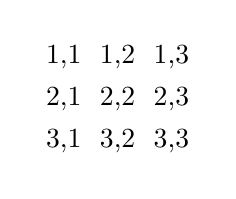
\begin{tikzpicture}



\custommatrix{beta}{3}{3}



% \begin{pgfonlayer}{background}
% \foreach \i in {1,2,3}
%   \foreach \j in {1,2,3}
%     \node[draw, thick, red, circle] at (m-\i-\j) {Top};
% \end{pgfonlayer}

\end{tikzpicture}
\end{document}